%\addcontentsline{toc}{chapter}{Development Process}
\chapter{Design}

\section{Overall Architecture}

\subsection{Class Descriptions}
\subsubsection{Game Classes}
The game class section will describe the different classes used within the project and where they link with the use of diagrams to help illlustrate.
\begin{figure}[h]
\centering
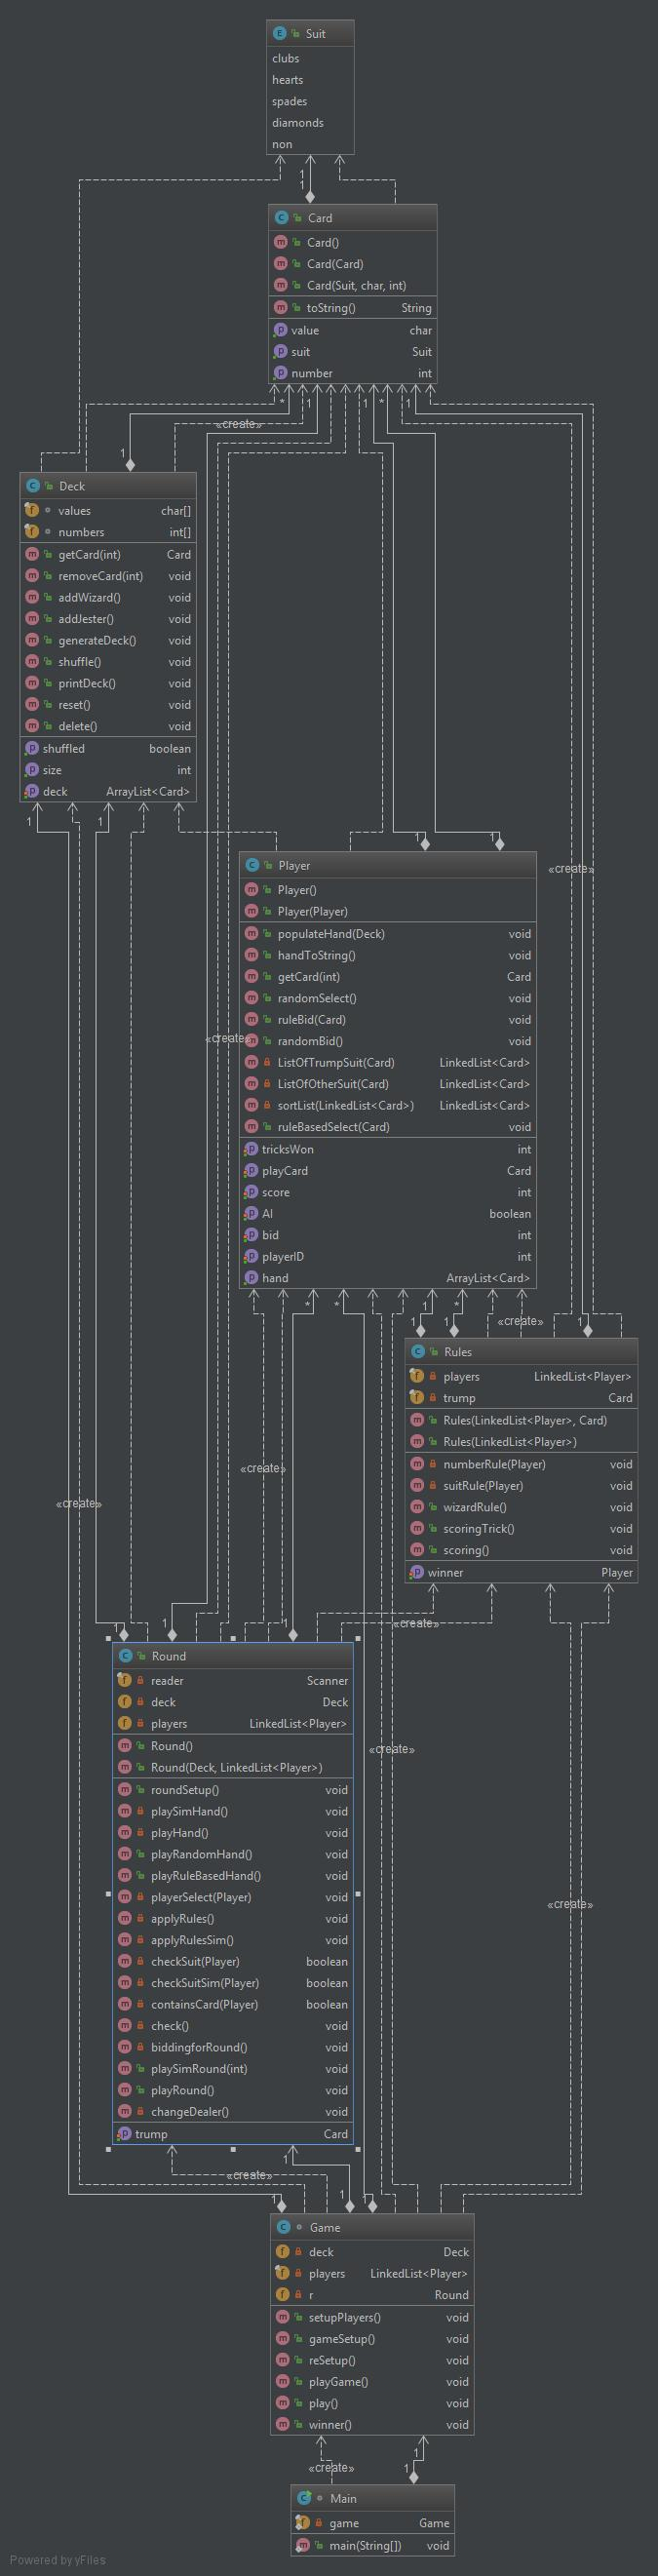
\includegraphics[width=15cm ,height=20cm,keepaspectratio]{Game_Classes}
\caption{Diagram Showing the Class Diagram of the Game Classes}
\label{fig:Game_Classes}
\end{figure}
\paragraph{Card}
This Card class created Card objects that will contain variables for the suit, the value of the card in relation to the other and the number displayed on the card such as a wizard or an ace. It will also contain methods to construct the card and getters and setters for each of the variables. Card will also contain a copying constructor for the use of the AI. This class will mainly be used in the generation of the deck but will also be used in the in other methods to refer to the suit and number(the value of the card in reference to the game, like ace being worth 14) used within the cards
\paragraph{Deck}
Deck is a class for create a deck object to be used for in the classes of game, round and the Monte Carlo Tree Search. It contains variables for an array of cards, and array of the different values there are for the cards and the numbers they each will have. There is also a Boolean variable to check if the deck has been shuffled. The deck class will also contain values to create and the wizards and jester cards to be added to the normal 52 card deck that is generated with a different method. there will also be a method to shuffle the deck of cards so that each player gets different cards for each round.
\paragraph{Player} 
The player class constructs the player objects that will contains variable for the player id; the cards they currently have in there hand; there bid and score; the card they have played for the trick; how many trick they have won and if it is an AI or normal player. This class will contain the getters and setts for the these variable whenever they will be need. It will also contain methods to print out the hand they currently have; constructors to copy the players variables; to populate the hand of the deck from cards they are within the deck. the is methods to randomly and rule based selection the cards and bids for the more simple AI.
\paragraph{Round}
The Round class will contains variable that are received from the game class and to be used in the Monte Carlo package and rules class. It will contain method to reset specific variables to setup and reset up the round. This classes method will also the player to play a card for the main game and the simulation use in the tree search. There will also be methods to change the dealer, applies the rules to the cards that are played and to check if the cards are valid to play.
\paragraph{Rules}
The rule class contains variables to show who was the winner for that rule it was using, the list of players and the trump card used in the round. It contains method to see, check and compare the suits and numbers of the player and if it is a wizard card they have player the automatically win for that trick. It also will contain a method to score the players based on how many trick they have won and how close they are to their bid. This will contain the variable collected from the round and game classes.
\paragraph{Game}
The game class contains methods to setup up the game with variables for the array of 3 players and how many are human, the round and the deck used. This class also contains methods to reset up the game, how many rounds are players and who the winner of the game is. 
\paragraph{Suit}
An enumerator class that contains the 5 different suits that the card could be such as heart, spades, clubs, diamonds and non for the wizard and jester cards.
\paragraph{Main}
This is the main class used to initialise the game and contains the game object for this to happen.
\subsubsection{Aritifical Intelligence Classes}
\begin{figure}[h]
\centering
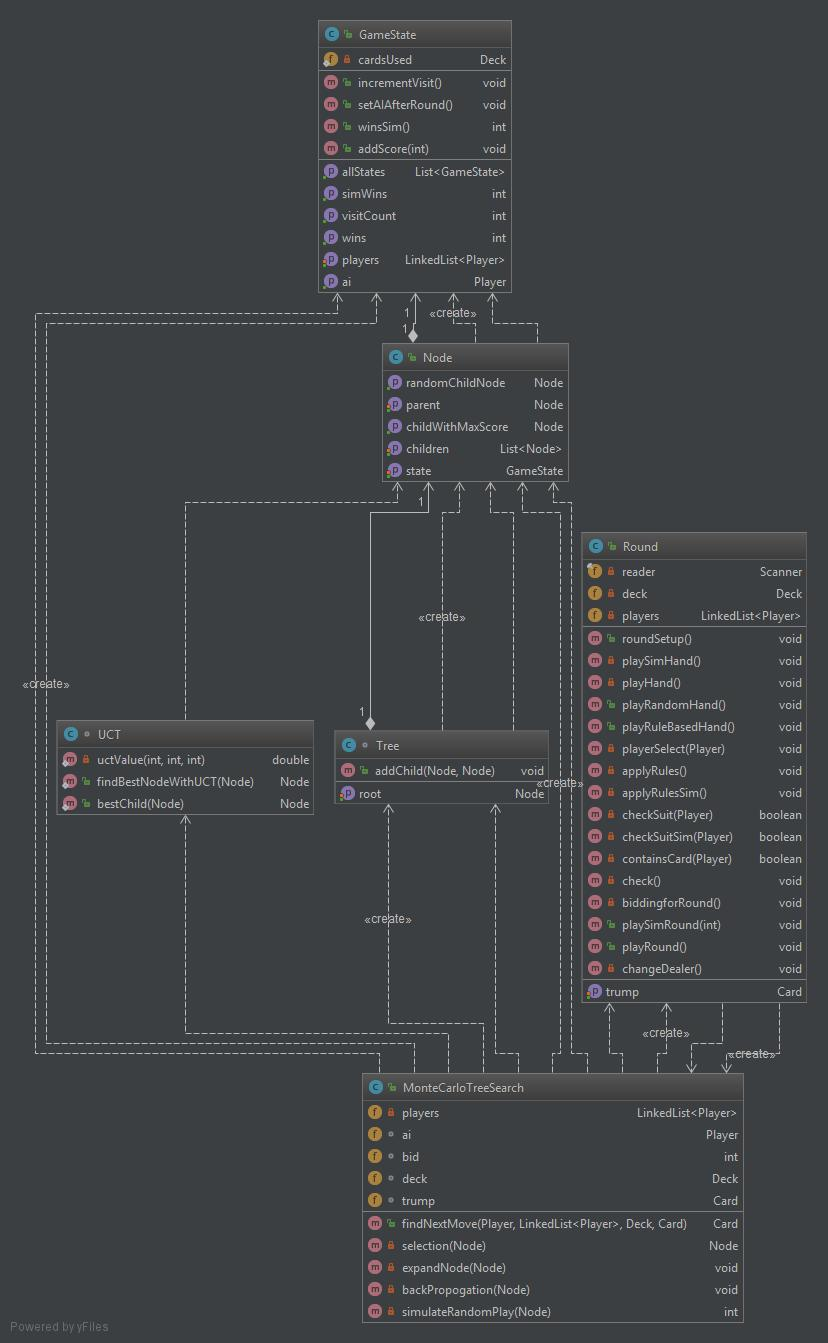
\includegraphics[width=15cm ,height=20cm,keepaspectratio]{AI_Classes}
\caption{Diagram Showing the Class Diagram of the AI Classes and the linking Round Class}
\label{fig:AI_Classes}
\end{figure}
This section will show you the classes associated with Monte Carlo Tree Search AI it made more sense for the complex Ai to be separate from the main game.
\paragraph{Node}
The node class contains the variables to see who it parent node is and list of its child nodes and the game state that contains the cards used by the players and their getters and setters. Node also contains the methods to randomly pick a child node and get a child of the node with the maximum score by comparing the ratio of simulation score to the amount of time the node has been visited.
\paragraph{Tree}
The tree node is for the use of starting the tree and contains one node of which is the root of the tree where all the nodes expand from. It will contain methods to get and set this root and add child to it.
\paragraph{GameState}
Game State is used to get the variables from the game in the state it is currently in when the tree search is used. The means there will need to be variable for the players, the amount of simulation the state has won in the node, the amount of times it has been visited and the trump card. The class will also contain getter and setters for these variables, with methods to increment the visits and to set a score based on the simulation in the tree search. There will also be a method that will give a list of possible states that the game may have meaning the play cards they the player may choose to have.
\paragraph{MonteCarloTreeSearch}
This is the main class that will choose the next card that the player will using the Monte Carlo tree search. It will be linked to all of the different classes within this package as well as the variables it uses from the round class that it will perform the findNextMove() method. This method will repeat the methods of selecting a promising nod; expanding this promising node; simulating the game and back propagation of the node for several iterations until a suitably large tree is created. This tree will then be used to select the best child node for selection of the play card.
\paragraph{UCT}
The UCT(Upper Confidence applied for trees) is the used in the selection of the nodes and select the next node to expand based on the total visits, node wins and node visits. this class will contain methods to find the best child by comparing these variables mentioned previously.
\section{Some detailed design}
In this section I will outline the important Algorithms to be used in the program and discuss how the User interface will looked and function.
\subsection{Algorithm Design}
The algorithm here will have Sequence diagrams to show the methods to be used to apply to the algorithms.
\subsubsection{Scoring}
The scoring algorithm give a score to each of the player in the game by multiply the amount of trick by 10. The value is then reduced by the difference between the number of tricks it has won and the initial bid the player has made. However, if the player has same amount of tricks won to their bid, they will gain an extra 20 points.
\begin{figure}
\centering
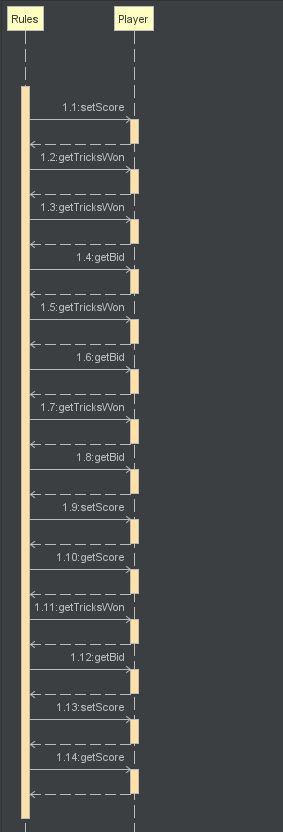
\includegraphics[width=15cm ,height=20cm,keepaspectratio]{ScoringSequenceDiagram}
\caption{Sequence Diagram of Scoring Method for Algorithm Description}
\label{fig:Scoring}
\end{figure}
\subsubsection{WinSim}
For this algorithms, it will give a based on how well the simulation has went for the player the MCTS is for. So if the score is equal to the bid it will be larger than if it was lower or higher than the bid.
\begin{figure}
\centering
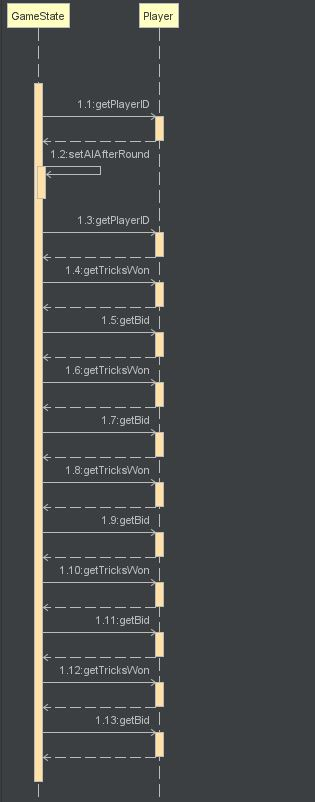
\includegraphics[width=15cm ,height=20cm,keepaspectratio]{WinSimSequenceDiagram}
\caption{Sequence Diagram of WinSim Method of Winning simulation Algorithm }
\label{fig:WinSim}
\end{figure}
\subsubsection{Rules}
For this algorithm, it will check to see if the player is a wizard or of the current winner is a winner. If current winner is it automatically wins. If not, it checks to see if it matches the trump suit or the dealers suit. If it does match the first players and is also trump it will check to see who has a higher valued cards and pick them as the winner but if it is a trump suit and the current winner isn’t then the new player will become the winner.
\begin{figure}
\centering
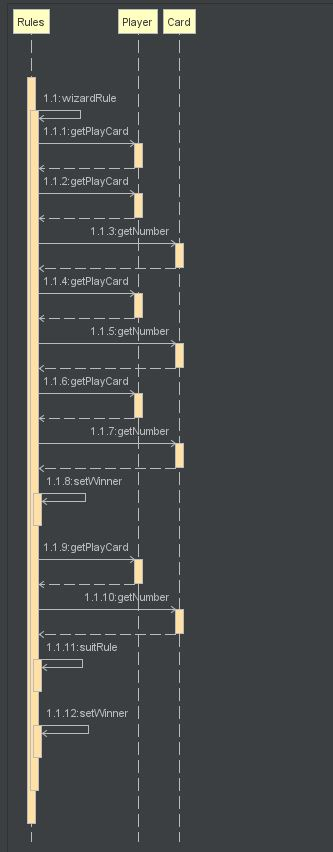
\includegraphics[width=15cm ,height=20cm,keepaspectratio]{RuleSequenceDiagram}
\caption{Sequence Diagram for the Rules Algorithm}
\label{fig:Rules}
\end{figure}
\subsubsection{Play Hand}
When the player is playing the hand, it will check to see if it is an AI or human player. If human, it will let the player select a card based on if it is a valid card to play. Otherwise, it is an AI, meaning the MCTS will be used to select the card. After this is will apply the rules to see who wins that specific trick.
\begin{figure}
\centering
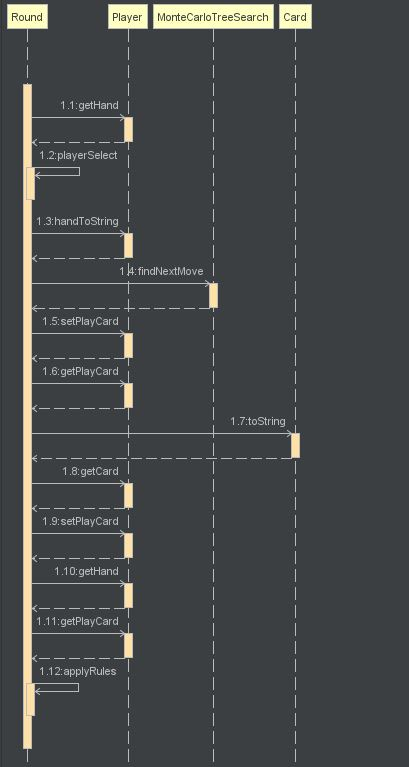
\includegraphics[width=15cm ,height=20cm,keepaspectratio]{PlayHandSequenceDiagram}
\caption{Sequence Diagram of Play Hand method for the Algorithm that shows what happens when a card is played}
\label{fig:Play}
\end{figure}
\section{User Interface}
As this project is mainly based on the Artificial Intelligence, only a simple User interface is needed. So, using a Terminal UI seems the best choice. This will include showing the cards that the player has in their hand and the card they will play. This interface will also allow you to bid at the beginning of the round after the trump card and hands have been given out. After the round has been completed it shows the number of tricks that has been won, the score they have received based on their bid and trick they have won.
